
Dans cette section nous nous intéressons aux problèmes d'ordonnancement proche de notre problème.
Définissons tout d'abord un problème d'ordonnancement :
\begin{mydef}
Un problème d'ordonnancement consiste à organiser des tâches dans le temps en respectant des contraintes temporelles et des contraintes de ressources.
\end{mydef} 
La composante d'ordonnancement est très présente dans les problèmes de \wsrp.
Les problèmes d'ordonnancement sont classifiés selon trois champs $\alpha~|~\beta~|~\gamma$.
Le champ $\alpha$ correspond aux contraintes sur les machines (nombre de machines, etc).
Le champ $\beta$ correspond aux contraintes entre les machines (précédence, préemption, etc) et aux contraintes de ressources.
Le champ $\gamma$ correspond à la fonction objectif que l'on veut optimiser (minimiser la complétion totale du planning, minimiser le retard des tâches, etc). 
Tous les champs appartiennent à $\alpha~|~\beta~|~\gamma$ sont détaillés dans le livre \cite{blazewicz2007handbook}.
Par exemple le problème $1~|~\textit{prec}~|~C_{max}$ correspond à l'ordonnancement de tâches sur une machine, les tâches ont des contraintes de précédences et on souhaite minimiser la complétion totale de l'ordonnancement.

Les problèmes d'ordonnancement sont regroupés dans la classe \ssp, cette classe a été définie par Graham et al. \cite{Graham1979}, ils présentent la complexité et les approximations de certains problèmes ; Lawler et al. \cite{Lawler1993} proposent des algorithmes pour résoudre ces problèmes.
\begin{mydef}
La classe \ssp ~est la classe des problèmes définis par l'allocation optimale de ressources rares pour des activités dans le temps.
La classe \ssp ~représente tous les problèmes d'ordonnancement classiques (ordonnancement sur une machine, ordonnancement de machines parallèles, OpenShop, FlowShop, JobShop, $\ldots$).
\end{mydef}

Les problèmes d'ordonnancement qui ressemblent le plus aux problèmes de la classe \wsrp ~sont les problèmes de la classe \mpsp (problème d'ordonnancement de projet à compétences multiples ou Multi-Skill Project Scheduling Problem en anglais). Les problèmes de la classe \mpsp ~consistent à trouver un ordonnancement réalisable des tâches en respectant les contraintes de précédence et de ressources : un employé/une machine peut effectuer une tâche que s'il/si elle possède les compétences et ressources requises.

Firat \cite{Firat2012} montre que le problème MPSP est $\np$-difficile, Blazewicz \cite{Blazewicz1983} montre que le problème d'ordonnancement de projet avec contrainte de ressources (resources constrainted project scheduling problem en anglais, noté RCPSP) est $\np$-difficile au sens fort. L’œuvre de synthèse  \cite{Graham1979} définit différents problèmes d'ordonnancement et leur approximation.

On retrouve des problèmes proches de ceux des \wsrp ~dans la littérature comme le problème de planning d'infirmières dans \cite{Trilling2007} ou dans \cite{Burke2010}.
L’œuvre de synthèse de Burke \cite{burke2004state} pose un état de l'art sur les problèmes de planning d'infirmières.
Le problème de planning d'infirmières est un problème qui possède beaucoup de contraintes souvent séparées en contraintes "molles" (soft constraints en anglais) qui peuvent être violées mais a un certain coût et contraintes "dures" (hard constraints en anglais) qui ne peuvent pas être violées. 
Les contraintes molles sont souvent les contraintes liées aux préférences des infirmières et les contraintes dures représentent les contraintes sur le temps de travail ou autres particularités qui sont assez réglementées.

La Figure~\ref{nurseRostering} montre un planning d'infirmières sur cinq jours avec deux sortes de "shifts" (early et late) avec des infirmières à temps plein et des infirmières à temps partiel et une demande de personnel pour chaque shift pour chaque jour.


\begin{figure}[H]
\centering
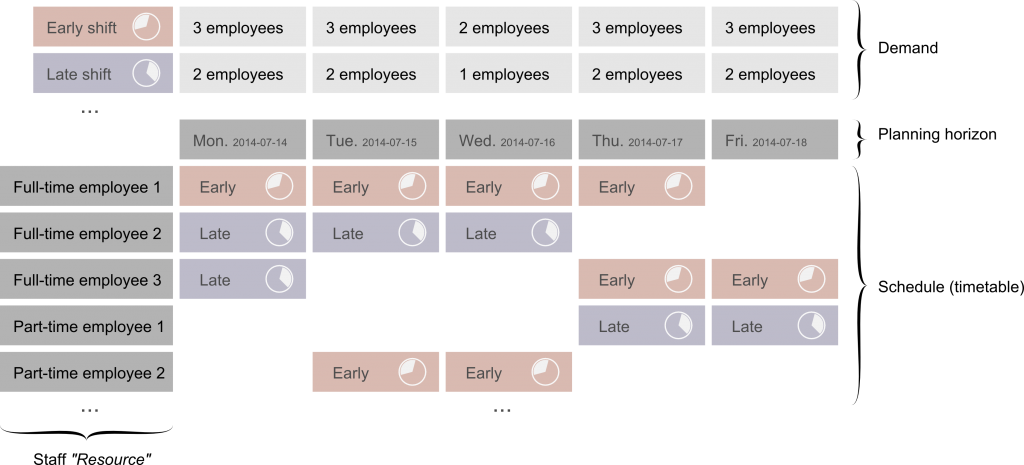
\includegraphics[scale=0.3]{nurseRostering.png}
\caption{Exemple de planning d'infirmières\label{nurseRostering}}
\end{figure}

Un autre problème d'ordonnancement proche des problèmes des \wsrp ~est le problème d'ordonnancement de techniciens et de tâches (\ttsp). \ttsp ~a été le sujet du challenge de 2007 de la ROADEF \cite{Cordeau2010,Pokutta2009,Hurkens2009}.
C'est un problème très présent dans le domaine de la télécommunication.
Dutot \cite{dutot2006technicians} définit le problème \ttsp. 
Hurkens et al.\cite{Hurkens2009} sont les vainqueurs de la compétition en utilisant la programmation linéaire mixte (Mixed Integer Programming) : ils utilisent une méthode de résolution en deux phases. 
La première pour obtenir de bonnes bornes inférieures et déterminer quelles tâches doivent être sous-traitées. 
La deuxième phase affecte les meilleurs couples tâche/technicien  en utilisant un algorithme de couplage.
Cordeau et al.\cite{Cordeau2010} finissent deuxième en utilisant des méthodes hybrides, programmation linéaire et heuristiques : recherche de voisinage large adaptatif \ref{def:ALNS}(Adaptative Large Neighborhood Search en anglais) et heuristique de construction.
Pokutta et al.\cite{Pokutta2009} terminent cinquième en se basant sur des méthodes heuristiques et de la recherche locale. 
Firat et al.\cite{Firat2012} améliorent la méthode de résolution de Hurkens et al.\cite{Hurkens2009} en trouvant de meilleures bornes inférieures dans la première phase. Ils obtiennent de meilleurs résultats. 

\begin{mydef}
\label{def:ALNS}
La recherche de voisinage large adaptatif (Adaptative Large Neighborhood Search en anglais) introduite par \cite{Ropke2005}, est une heuristique qui étend la méta-heuristique Large Neighborhood Search proposée par \cite{shaw1998using} et est très proche de l'heuristique de destruction et de réparation de \cite{schrimpf2000record}. Le comportement de l'heuristique est le suivant : en partant d'une solution initiale, on dégrade/détruit une partie de la solution pour ensuite la reconstruire de manière optimale (localement). En enchaînant successivement ces deux étapes, on espère obtenir une solution de meilleure qualité. Cette méthode a d'abord eu de nombreux succès pour les problèmes de routage, puis s'est étendue vers de nombreux autres problèmes comme les problèmes d'ordonnancement.
\end{mydef}
